% change according to folder and file names
\ifpdf
    \graphicspath{{4/figures/PNG/}{4/figures/PDF/}{3/figures/}}
\else
    \graphicspath{{4/figures/EPS/}{4/figures/}}
\fi

%: ----------------------- contents from here ------------------------
\chapter{Variable-correlation driven EA} % top level followed by section, subsection
%\begin{flushright}
%Any intelligent fool can make things  
%\linebreak
%bigger, more complex, and more violent. 
%\linebreak
%It takes a touch of genius, and a lot of  
%\linebreak
%courage, to move in the opposite direction.
%\linebreak
%Albert Einstein
%\end{flushright}

This Chapter investigates the behaviour of EAs (MAEAs) on ill-conditioned not-separable functions. It is proven that the performance of EAs significantly deteriorates when they are dealing with ill-conditioned optimization problems with not-separable design variables \cite{Salomon,Roy_2002a,Ghisu_2010}. Herein the combination of ill-conditioning and not-separability will be referred to as variable correlations. Unfortunately, in their majority, engineering optimization problems belong in this category. Furthermore this Chapter proposes and validates a novice method to regain a major part of the lost, dew to variable correlations, EA efficiency.  

\section{Objective function difficulties}
In order to devise a method that regains the lost efficiency due to variable correlations we first have to investigate and understand where this difficulties arose from. This difficulties can be seen as difficulties origin from the objective function/s since they solely relay on the shape of the objective function/s in the design space (correlation between the objective function and the design variables). In the following two objective function properties, ill-conditioning and not-separability, that combined lead to variable correlation and thus significantly reduce EA efficiency will be presented.

\subsection{Ill-conditioning}
\label{IllCon}
Regarding variable correlation, the term ill-conditioned refers to the condition were the contribution to the objective function value is largely non-homogeneous for the different design variables or ,more precisely, directions in search space.

\begin{figure}[h!]
\begin{minipage}[b]{0.5\linewidth}
 \centering
 \resizebox*{9cm}{!}{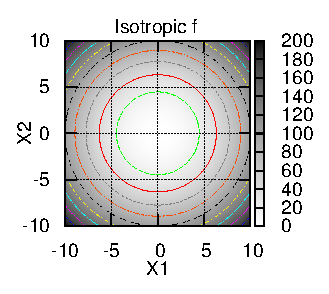
\includegraphics{sphere.eps}}
\end{minipage}
\begin{minipage}[b]{0.5\linewidth}
 \centering
 \resizebox*{9cm}{!}{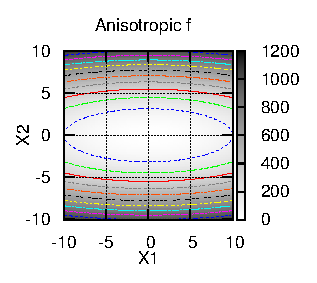
\includegraphics{ellipse.eps}}
\end{minipage}
\caption{Left: Well-conditioned objective function with two design variables; the contribution of both $X_1$ and $X_2$ are the same. Right: Ill-conditioned objective function; variable $X_2$ has higher contribution on the objective function than $X_1$.} 
\label{illc}
\end{figure}

In practise EAs are sophisticated enough to deal with ill-conditioned problems without loosing efficiency. Ill-conditioned objective functions, though, are prune to non-separability.         


\subsection{Non-separability}    
Separability of an objective function $f:\vec{x}\mapsto f(\vec{x})$ is the condition described for each and every variable $x_i \in \vec{x}$. An objective function is said to be separable with respect to $x_i$ if the optimal value of $x_i$ does not depend on the choice of the remaining design variables. Furthermore an objective function $f$ i said to be separable if it is separable with respect to each and every member of $\vec{x}$.


\begin{figure}[h!]
\begin{minipage}[b]{0.5\linewidth}
 \centering
 \resizebox*{9cm}{!}{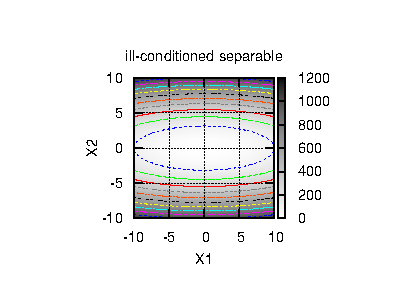
\includegraphics{ellipse2.eps}}
\end{minipage}
\begin{minipage}[b]{0.5\linewidth}
 \centering
 \resizebox*{9cm}{!}{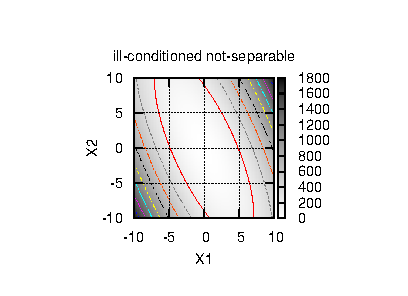
\includegraphics{ellipseturn.eps}}
\end{minipage}
\caption{Left:  Right:.} 
\label{nonsep}
\end{figure}

Optimization problems with non-separable objective functions are subject to the curse of dimensionality. Regarding non-separable objective functions, difficulty scales exponentially fast with the dimension since the search space volume also increases exponentially with the dimension, leading to the notion of curse of dimensionality. On the other hand separable objective functions, even though the search space volume also increases exponentially, their difficulty scales only linearly with the search space dimension thus they are not subject to the curse of dimensionality since the global optimum could be located by minimizing $n$ one dimensional objective functions (minimise $f_i(x_i),~ \forall x_i \in \vec{x}$).
 
\subsection{Investigation of the effects of Variable correlations on EA efficiency}

In order to Investigate the effects of variable correlations on EA efficiency two analytical test cases have been solved, for a range of design space dimensions, both in their separable and non-separable form.

The first analytical test case to me examined is a multidimensional ellipsoid (a 2d version of it can be seen in fig. \ref{nonsep}) described, in it separable form, by:   


\begin{eqnarray}
   f(\vec{x})=\sum^{n}_{i=1}=a^{\frac{i-1}{n-1}}x_i^2
   \label{ellipse} 
\end{eqnarray}
where $a$ is the so called condition number and controls the ill-conditioned state of the objective function. Large values of $a$ lead to increasingly ill-conditioned objective functions.

and in its non-separable form by:

\begin{eqnarray}
   f(\vec{x})=\sum^{n}_{i=1}=a^{\frac{i-1}{n-1}}y_i^2
   \label{ellipse} 
\end{eqnarray}
where $\vec{y}=B\vec{x}$ and $B$ a $n\times n$ orthogonal, rotation, matrix.

In order to investigate both the effects of the design space dimension ($n$) and the condition number ($a$) four different optimization problems will be solved. A ten dimensional ($n=10$) optimizations problem is solved for $a=10$ and $a=1000$, see fig. \ref{ellipse_t1}, and a $n=30$ problem is solved for $a=100$ and $a=1000$, see fig. \ref{ellipse_t1}, 


\begin{figure}[h!]
\begin{minipage}[b]{0.5\linewidth}
 \centering
 \resizebox*{7cm}{!}{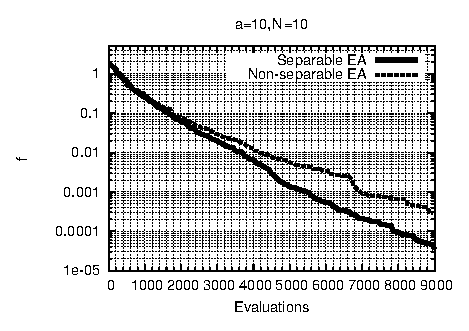
\includegraphics{10_10d.eps}}
\end{minipage}
\begin{minipage}[b]{0.5\linewidth}
 \centering
 \resizebox*{7cm}{!}{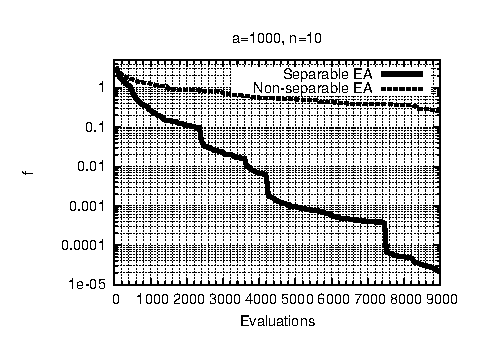
\includegraphics{1000_10d.eps}}
\end{minipage}
\caption{Ten dimensional ellipsoid. Left: Condition number ($a=10$).  Right: Condition number ($a=1000$). For both cases, $a=10$ \& $a=1000$, significant losses in efficiency due to variable correlations (non-separability) are observed. Furthermore both for the separable and non-separable problem the increase of $a$ for $10$ to $1000$ causes additional losses.} 
\label{ellipse_t1}
\end{figure}

\begin{figure}[h!]
\begin{minipage}[b]{0.5\linewidth}
 \centering
 \resizebox*{7cm}{!}{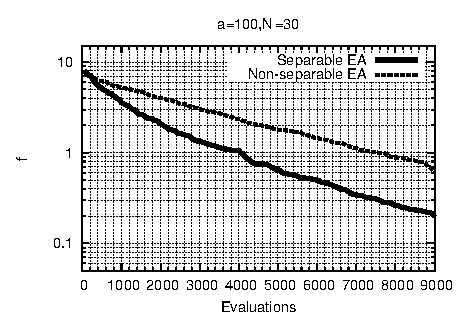
\includegraphics{100_30d.eps}}
\end{minipage}
\begin{minipage}[b]{0.5\linewidth}
 \centering
 \resizebox*{7cm}{!}{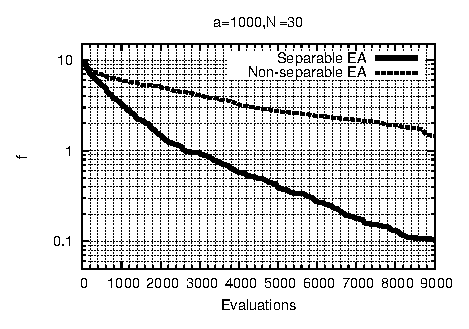
\includegraphics{1000_30d.eps}}
\end{minipage}
\caption{30 dimensional ellipsoid. Left: Condition number ($a=100$).  Right: Condition number ($a=1000$). For both cases, $a=10$ \& $a=1000$, significant losses in efficiency due to variable correlations (non-separability) are observed. Condition numbers of $100 - 1000$ demonstrate similar convergence.} 

\label{ellipse_t2}
\end{figure}

\newpage
The second analytical test case to me examined here is a multidimensional multi-modal objective function described by:  

\begin{eqnarray}
   f(\vec{x})=10*n+(\sum^{n}_{i=1}x_i)^2 - 10*n*cos(\pi * \sum^{n}_{i=1}x_i)
   \label{mm} 
\end{eqnarray}

A two dimentional example of it can be found in fig. \ref{multimod}. The above problem, in the eq. \ref{mm} form, is non-separable as shown in fig. \ref{multimod}. It can though easily be transformed to a separable one if $\vec{x}$ is transformed into $\vec{y}$ through the operation $\vec{y}=B\vec{x}$ where $B$ the rotation matrix with its first raw equal to the unity vector ($45^o$ rotation $\forall$ directions).  This objective function can also be classified as extremely ill-conditioned since only one of the separable directions has contribution in the objective faction value and all the rest became irrelevant. This is an important class of objective functions since it resembles MOO problems as we will see further on (\ref{VCMM}).    

In order to investigate the effects of non-separability as a function of the problems dimension two optimization problems where solved a $5$ and a $30$ dimensional one.  
\begin{figure}[h!]
\begin{minipage}[b]{0.5\linewidth}
 \centering
 \resizebox*{7cm}{!}{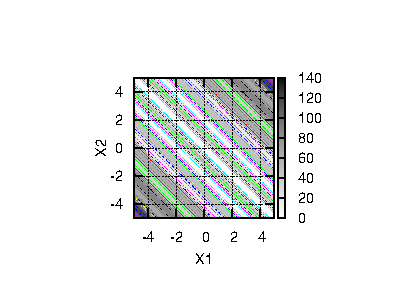
\includegraphics{multimod.eps}}
\end{minipage}
\begin{minipage}[b]{0.5\linewidth}
 \centering
 \resizebox*{7cm}{!}{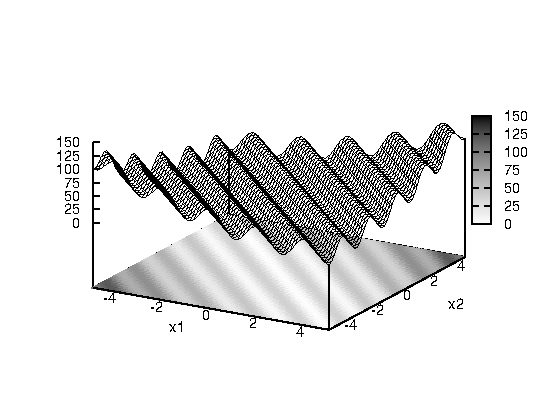
\includegraphics{multimodnomap.eps}}
\end{minipage}
\caption{Two dimensional example of the optimizations problem eq. \ref{mm}. In this example optimum value of $x_1$ is depended of the choice of $x_2$ and vice versa thus this objective function suffers from variable correlations (non-separable). If, nevertheless, one of the two design variables was aligned to the $x_1+x_2$ axis, or the $\sum^{n}_{i=1}x_i$ one in the $n$ dimensional case, the problem becomes separable.} 

\label{multimod}
\end{figure}


\begin{figure}[h!]
\begin{minipage}[b]{0.5\linewidth}
 \centering
 \resizebox*{7cm}{!}{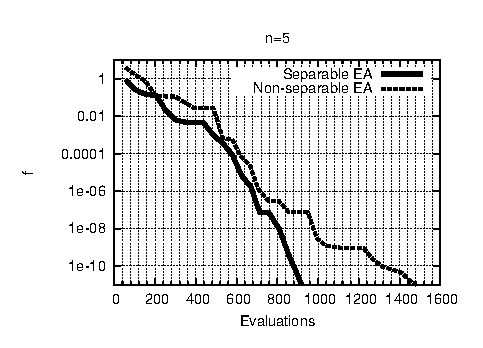
\includegraphics{5d.eps}}
\end{minipage}
\begin{minipage}[b]{0.5\linewidth}
 \centering
 \resizebox*{7cm}{!}{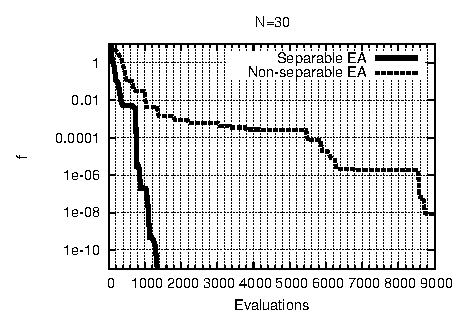
\includegraphics{30d.eps}}
\end{minipage}
\caption{Left: 5 dimensional optimization problem eq.\ref{mm}. Right: 30 dimensional optimization problem eq.\ref{mm}. The amount of efficiency losses in problems with extremely ill-conditioned objective functions increases significantly with the dimension of the design space.} 
\label{multimodres}
\end{figure}

Through the investigations of the effects of variable correlation presented in figs. \ref{ellipse_t1}, \ref{ellipse_t2} and \ref{multimodres} it is proven that a significant amount of EA effitiency can be lost when they are dealing with optimization problems with correlated design variables. The severity of efficiency deterioration is analogous to three main quantities;

\begin{description}
  \item[a)] The condition number, which is a measure of the non-homogeneous contribution of each design variable on the objective function thus a measure of the condition state of the problem in hand \ref{IllCon}. The bigger the condition number gets the bigger loss of EA efficiency is observed (fig. \ref{ellipse_t1}). For very big condition numbers $>100$ the efficiency losses due to ill-conditioning remain stable at their maximum possible value (fig. \ref{ellipse_t2}).    
  \item[b)] Separability. Optimization problems with separable design variables can be solved significantly faster, using an EAs, as it is shown in figs. \ref{ellipse_t1}, \ref{ellipse_t2} and \ref{multimodres}.  
  \item[c)] The number of design variables $n$. Though it is obvious that increasing the number of design variables will also increase the design space thus require more resources for any stochastic search algorithm to locate the optimum solution, what is of interest in this section is that by increasing $n$ the losses generated from non-separability are magnified (fig. \ref{multimodres}).  
\end{description}
\section{Variable correlations in MOO}
\label{VCMM}
Regarding design variable correlations in MOO problems one should observe the shape of the scalar cost faction $\Phi$, since this is the value that controls the evolution operators, and not each and every objective function separably. In MOO variable correlations are typically in the form of non-separable extremely ill-conditioned state. This results from the fact that a Pareto front of optimal non-dominated solutions is sought. If the $\Phi$ assignment technique is based on Pareto dominance all members of the current front of non-dominated solutions have $\Phi=0$ (or very small values compared to the dominated members of the population) thus;
\begin{eqnarray}
   \mbox{Pareto front} \Rightarrow 	\Phi(\vec{f})=0  
   \label{Corr-Par} 
\end{eqnarray}
because $\vec{f}=\vec{f}(\vec{x})$,
\begin{eqnarray}
	\Phi(\vec{f}(\vec{x}))=0 \Rightarrow \Phi^*(\vec{x})=0
    \label{Corr-Par2}
\end{eqnarray}
where $\Phi^*$ is the direction in design space with the bigger variance.

An analytical form of $\Phi^*$ is, in the general case, very difficult to calculate due mainly to the non analytical form of $\Phi$ (eq.\ref{SPEAIIeq}) and the complex mapping form objective space to design variable space. In this thesis a method that can estimate, with increasing accuracy as the evolution proceeds, the variable correlations without calculating the analytical form of $\Phi^*$ is proposed. Further more new evolution operators are proposed to utilize this information in an EA frame.  

%\begin{figure}[h!]
%\begin{minipage}[b]{1\linewidth}
% \centering
% \resizebox*{10cm}{!}{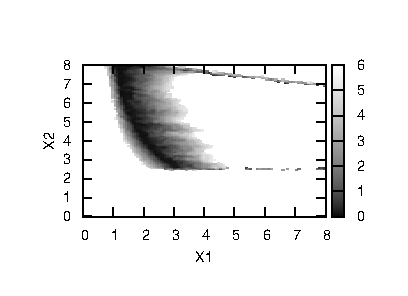
\includegraphics{CaseCorr.eps}}
%\end{minipage}
%\caption{Example $\Phi'$ plot for} 
%\label{phi1}
%\end{figure}
\section{Variable correlation estimation}
Since the current front of non-dominated solutions "elite-set" ($\Phi=0$) is the best so far approximation of the actual Pareto front it can be used to estimate the variable correlations. This estimations are as close to the real correlations as close as the current elite-set is to the actual Pareto front. Therefore dynamically updated variable correlations estimation as the elite-set increases in quality is proposed. To extract the internal structure of the elite-set in the design variable space without computing an analytical formula and in a way which best explains the variance principal component analysis (PCA) is used. 
 
PCA is an eigenvector--based multivariate analysis, performed on a data--set, that transforms possibly correlated variable sets into uncorrelated ones known as principal components. The latter are the direction vectors that best represent the variance in the data--set, \cite{Haykin,Jolliffe_2002}.
 
By assuming the current elite set to be a standardized data--set ($X$) with the empirical covariance matrix, \cite{Fodor_2002, Jolliffe_2002},

\begin{equation} 
   P_{N\times N}= \frac{1}{e}XX^T
   \label{Cov_Mat} 
\end{equation}
where $e$ is the size of $S_e$, we can use the spectral decomposition theorem, \cite{Axler_1997, Fodor_2002}, to write $P$ as

\begin{equation} 
   P_{N\times N}= U\Lambda U^T
   \label{spectral}
\end{equation}
where $\Lambda\!=\!diag(\lambda_1 , . . . , \lambda_n )$ is the diagonal matrix with the eigenvalues of $P$ and $U$ is a $N\!\times\!N$ matrix containing the eigenvectors also known as principal components or directions. 

In this PhD thesis it is proposed that the principal directions, as they are computed via PCA on the elite-set in order to best represent the variance in it, are also the directions in the search space that have the biggest degree of separability between them as far as the optimization problem in hand is concerned 

To better demonstrate the variable correlation estimation in MOO problems  the welded beam test case is used.  

\begin{figure}[h!]
\begin{minipage}[b]{1\linewidth}
 \centering
 \resizebox*{!}{4.5 cm}{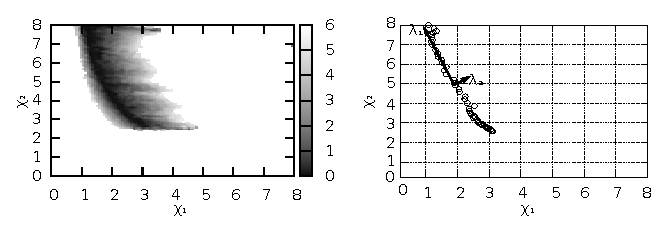
\includegraphics{DOFs.eps}}
\end{minipage}
%\begin{minipage}[b]{0.5\linewidth}
% \centering
%\resizebox*{8cm}{!}{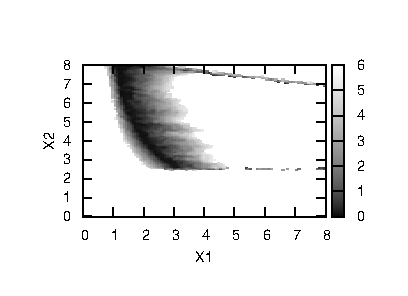
\includegraphics{CaseCorr.eps}}
%\end{minipage}
\caption{Example $\Phi'$ plot. $\Phi' = 0$ suggest the presence of CDV in the form of $X_1=-X_2$.} 
\label{reco1}
\end{figure}


\section{PCA driven evolution operators} 
PCA driven evolution operators to better ``drive'' evolution by utilising the information about the design variable correlations is proposed here as a method to deal with non-separable \& ill-conditioned optimization problems. To be more specific, PCA is used to identify the relations in the form of direction in the design space. The design space is, then, temporarily aligned with these directions, the necessary evolution operators apply to the so--rotated individuals and, finally, the generated offspring are transformed back to the original design space. Any sort of dimensionality reduction or rotation of the design space occurs just before (and after) the application of the evolution operators. To initiate PCA, a small number of representative solutions to the problem must be available; this set is dynamically updated during the evolution. In MOO applications, this comprises the members of the current front of non--dominated solutions. In SOO problems, in which there is no set of non--dominated solutions, the principal components can be found by processing a user--defined number of top individuals in the current offspring population. It is evident that, as the evolution proceeds, and the current front of non--dominated solutions converges to the Pareto front, the principal components approach those of the Pareto front. 

Let the aligned to the principal components design vectors \(\overrightarrow{x_i}\) be represented by \(\overrightarrow{x^*_i}\). The alignment is performed as follows
\begin{equation} 
   \overrightarrow{x^*_i}=U(\overrightarrow{x_i}-\mu_{X})
   \label{align} %http://users.ics.tkk.fi/jhollmen/dippa/node30.html
\end{equation}
where $\mu_{X}$ is the vector of mean (over the elite set) design variables.
The inverse transformation, from $x^*_i$ to $x_i$, is given by
\begin{equation} 
   \overrightarrow{x_i}=U^{-1}\overrightarrow{x^*_i}+\mu_{X}
	\label{re-align}
\end{equation}
It is important to note that the CPU cost to compute \(U^{-1}\) is negligible since U is an orthogonal matrix and, thus, \(U^{-1} = U^T\). 

The two main PCA driven evolution operators, recombination and mutation, are presented below.  

\paragraph{}
\subsection{PCA driven recombination}
In PCA driven recombination the evolution operator is applied on a continuously updated design space which is sought to be as separable as possible. In fig.\ref{reco1}-left the $\Phi$ of given MOO problem is plotted .    

\begin{figure}[h!]
\begin{minipage}[b]{0.5\linewidth}
 \centering
 \resizebox*{8cm}{!}{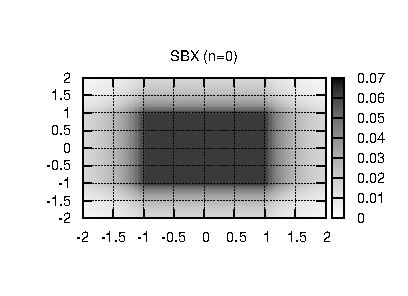
\includegraphics{SBX3dparents2.eps}}
\end{minipage}
\begin{minipage}[b]{0.5\linewidth}
 \centering
 \resizebox*{8cm}{!}{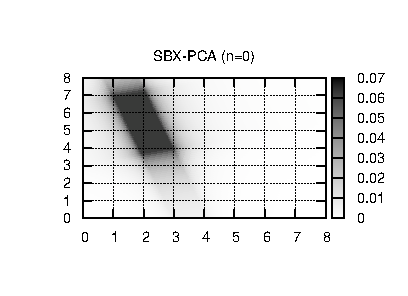
\includegraphics{SBX3dparents2PCA.eps}}
\end{minipage}
\caption{Example $\Phi'$ plot. $\Phi' = 0$ suggest the presence of CDV in the form of $X_1=-X_2$.} 
\label{reco2}
\end{figure}
\pagebreak
%\begin{figure}[h!]
%\begin{minipage}[b]{1\linewidth}
% \centering
% \resizebox*{10cm}{!}{\includegraphics{ellipseturn_eig.eps}}
%\end{minipage}
%\caption{Example $\Phi'$ plot for} 
%\label{phi1}
%\end{figure}


\subsection{PCA driven mutation}
In MAEA(PCA) mutation is applied on the aligned with CDV directions design space. Mutation probability on each CDV direction is dynamically updated based on the variance ($\vec{V}$) among the members of the elite population on the aforementioned direction ($V(i)$) eq.\ref{alignMut}.    

\begin{equation} 
   P_m^{i}=0.1 P_m + \frac{0.9 P_m N}{P_m^{gl}} (1-\frac{(V(i)-min(\vec{V}))}{(max(\vec{V})-min(\vec{V}))}),~~~~i=1,N 
   \label{alignMut} %http://users.ics.tkk.fi/jhollmen/dippa/node30.html
\end{equation}
where $P_m$ is the user-defined mutation probability, N the number of design variables and 
\begin{equation} 
   P_m^{gl}=\sum^{N}_{i=1} 1-\frac{(V(i)-min(\vec{V}))}{(max(\vec{V})-min(\vec{V}))}
   \label{alignMut2} %http://users.ics.tkk.fi/jhollmen/dippa/node30.html
\end{equation}
%%%%%%%%%%%%%%%%%%%%%%%%%%%%%%%%%%%%%%%%%
{\bf The PCA--driven MAEA (MAEA(PCA)) fig.\ref{MAEAPCA2} :}
%%%%%%%%%%%%%%%%%%%%%%%%%%%%%%%%%%%%%%%%%

Let us denote the generation counter by $g$, the number of current entries into the DB by $k_{DB}$ and the minimum number of entries needed to initiate the use of the metamodel--based pre--evaluation phase by $k_{min}$. Then, the steps of the PCA--driven MAEA can be described as follows:
\begin{description}
  \item[Step 1:] For the current offspring population $S^{g}_\lambda$, set $\lambda^*\!=\!\lambda$ (if $k_{DB}\!<\!k_{min}$) or  $\lambda^*\!=\!\lambda_{ex}$ (else). 
  \item[Step 2:] If $k_{DB}\!\ge\!k_{min}$, train $\lambda$ RBF networks on paired input--output patterns selected from the DB, in the vicinity of each offspring. Pre--evaluate the $\lambda$ population members on the so--trained metamodels. Select the $\lambda_{ex}$ top of them, based on dominality and proximity criteria.
  \item[Step 3:] Evaluate the $\lambda_{ex}$ offspring on the problem--specific evaluation software. Update $S^{g}_e$.
  \item[Step 4:] Compute the current set of principal components based on the updated elite set $S^{g}_e$ (eqs. \ref{Cov_Mat} and \ref{spectral}).
  \item[Step 5:] Align the design space to so--computed principal components (eq. \ref{align}). 
  \item[Step 6:] Create the new offspring population $S^{g+1}_\lambda$ through the application of the evolution operator on the aligned individuals. Re--align the generated offspring to the original design space coordinate system,(eq.~\ref{re-align}).
  \item[Step 7:] Set $g\!\leftarrow\!g\!+\!1$; go to step 1.
\end{description}
The above algorithm can readily be transformed to EA(PCA) by eliminating the use of metamodels or by setting $k_{min}$ to a practically infinite number.  To transform the objecive function vectors into scalar quantities, SPEA2 (\cite{kn:Zitz02}) is used; however, this is not restrictive at all.

In order to demonstrate the possible performance gain from the use of the PCA--driven EA ten runs for the aforementioned (Welded beam) case was performed with different random number generator seeding. The average hypervolume indicator in respect to evaluations, over the ten runs, is presented in fig. \ref{HypervolumeComparison}.

\figuremacroW{HypervolumeComparison}{Hypervolume Comparison}{Hypervolume comparison between EA and EA(PCA), metamodels where not used due to the fast evaluation time of the welded beam case. EA(PCA) outperforms traditional EA even though the dimensionality of the problem in hand is very low.}{0.9}

\figuremacroW{MAEAPCA2}{MAEA-PCA}{Schematic representation of the PCA-driven MAEA algorithm.}{1.0}


\section{PCA assisted metamodels}
The use of IPE suffers from the curse of dimensionality, with increased dimension both the prediction accuracy decreases and the training time (in case of ANN) increases. Here a method is proposed in order to reduce the $\vec{x}$ dimension in a favourable for the optimization way. As mentioned above the variable correlations are extracted via PCA performed on the members of the elite population in the form of eigenvectors, directions in the design space, and eigenvalues, variance of the corresponding direction. If a direction has big variance it means that the members of the elite population are scattered over a big range on it, that implies that this direction is of low importance for the optimization procedure. On the other hand if a direction has small variance that means that the members of the elite population are concentrated in a small region thus the direction is of big importance for the optimization.        

Since the Variable-correlations have been detected through PCA performed on the members of the elite population they could also be used to assist the metamodel training via reducing the $\vec{x}$ dimension. It is a well known fact that metamodels suffer from the curse of dimensionality, in case of RBFn with increased dimension both the prediction accuracy decreases and the training time increases. To treat this 

in the form of eigenvectors, denoting directions in the design space, and eigenvalues, denoting the variance of the elite population members in the corresponding direction. 

\section{Welded beam demonstration case}
The presence and exploitation of relationships between decision variables will be demonstrated through a known simple case, namely the minimization of both the cost ($K$) and the deflection ($\Delta$) of a welded beam subject to a force $P$ (fig. \ref{case}). There are two design variables: the side length of the square cross section ($X_2$) and the welding length ($X_1$) (fig. \ref{case}). The design is made subject to constraints o shear stress ($\tau$), bending stress ($\sigma$) and buckling load ($P_c$).   

\figuremacroW{case}{Welded beam case - Problem definition.}{In the examined case, design variables are square cross section side-length ($X_2 = t$) and welding length ($X_1 = l$) are the design variables.}{0.4}

The problem can be formulated as,

Minimize Cost,
%\begin{equation} 
\begin{eqnarray}\nonumber
   K = 1.10471h^2l+0.04811t^2(14.0+l) \\
   = 1.10471h^2X_1+0.04811X_2^2(14.0+X_1)
   \label{Cost} 
\end{eqnarray}
and minimize Deflection,
%\end{equation}
\begin{eqnarray}
   \Delta = \frac{4PL^3}{Et^4} = \frac{4PL^3}{EX_2^4}
   \label{Deflection} 
\end{eqnarray}

Subject to:


Constraint concerning the shear stress applied on the welding in order to ensure the structural integrity of the welding. Maximum shear stress depends on the type and quality of the welding. 
\begin{eqnarray}
   \tau = \sqrt{\tau_1^2 + \frac{\tau_1 \tau_2 l}{R} +\tau_2^2} \\
   \nonumber \tau \leq 13,600 psi \\
   \nonumber where:~~~~~~~~~~~~~~~~~~~~~~.\\
   \nonumber \tau_1 = \frac{P}{\sqrt{2}hl} \\
   \nonumber \tau_2 = \frac{MR}{J} \\   
   \nonumber M = P(L+\frac{l}{2}) \\ 
   \nonumber R = \sqrt{\frac{l^2}{4} + (\frac{h+t}{2})^2} \\
   \nonumber J = 2\left( \sqrt{2}hl\left( \frac{l^2}{12} + \left(\frac{h+t}{2}\right)^2 \right) \right)
   \label{shear} 
\end{eqnarray}

concerning the bending stress applied on the beam, to ensure structural integrity of the beam. Maximum bending stress depends on the beam material.
\begin{eqnarray}
   \sigma = \frac{6PL}{t^3} \leq 30,000 psi
   \label{bend} 
\end{eqnarray}

and concerning the buckling load, to avoid buckling phenomena.  
\begin{eqnarray}
   P_c = \frac{4.013E\sqrt{\frac{t^8}{36}}}{L^2}\left( 1- \frac{t}{2L}\sqrt{\frac{E}{4G}} \right) \\
   \nonumber  P - P_c \leq 0 
   \label{back} 
\end{eqnarray}
,where welding hight is $h = 0.6 in$, beam reach is $L = 14 in$, the extend of the force is $P = 6000 lb$, Young’s modulus is $E = 30 \times 10^6 psi$, and shear modulus is $G = 12 \times 10^6 psi$.  

Apart from the structural, constraints are also enforced on the objectives to bound the Pareto front within logical values, thus:

\begin{eqnarray}
   K \leq 50 \\
   \Delta \leq 0.25 
   \label{obj} 
\end{eqnarray}


\begin{figure}[h!]
\begin{minipage}[b]{0.5\linewidth}
 \centering
 \resizebox*{7.5cm}{!}{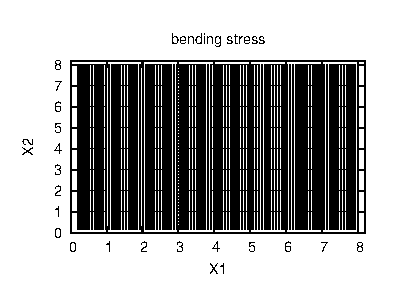
\includegraphics{Const_sx.eps}}
\end{minipage}
\begin{minipage}[b]{0.5\linewidth}
 \centering
 \resizebox*{7.5cm}{!}{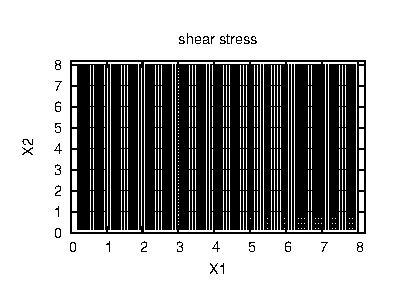
\includegraphics{Const_tx.eps}}
\end{minipage}
\begin{minipage}[b]{0.5\linewidth}
 \centering
 \resizebox*{7.5cm}{!}{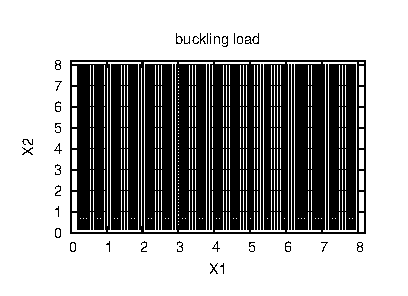
\includegraphics{Const_P.eps}}
\end{minipage}
\begin{minipage}[b]{0.5\linewidth}
 \centering
 \resizebox*{7.5cm}{!}{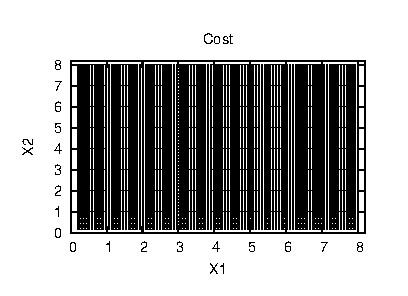
\includegraphics{Const_Price.eps}}
\end{minipage}
\begin{minipage}[b]{0.5\linewidth}
 \centering
 \resizebox*{7.5cm}{!}{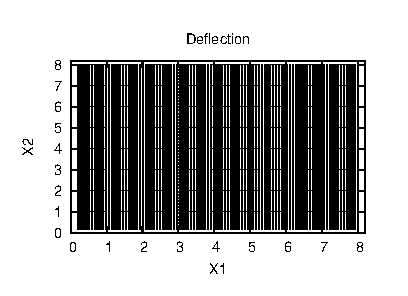
\includegraphics{Const_Dx.eps}}
\end{minipage}
\begin{minipage}[b]{0.5\linewidth}
 \centering
 \resizebox*{7.5cm}{!}{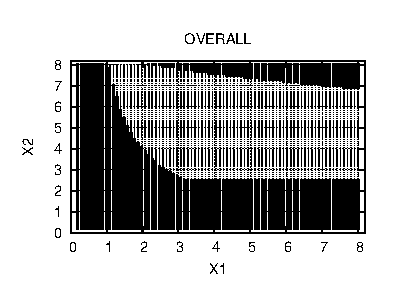
\includegraphics{Const_ALL.eps}}
\end{minipage}

\caption{Investigation of the feasibility of the design $(X_1,X_2)$ plane. The overall feasible design space is presented in the lower right figure with white squares. Constraints buckling load and maximum deflection  are both overpowered by bending stress and could be eliminated.} 
\label{x1x2}
\end{figure}


\paragraph{}
This case was deliberately chosen as a demonstration case due to the clear physical meaning of the relations that appear between its design variables. By carefully examining the objectives it is clear that in order to decrease deflection $X_1$ must be increased(eq. \ref{Deflection}). However any increase in $X_1$ will lead to higher cost (eq. \ref{Cost} ). In order to keep cost stable $X_2$ must simultaneously decrease, this of-course is bounded by the structural constraints (eq. \ref{shear},\ref{bend} and \ref{back}). 
 
This type of relations appear in all multiobjective cases. As long as a Pareto front is sought then a relation between the objectives exist $G(F_1,F_2)=0$ (fig. \ref{pareto_DOFs} -right) and since $F_i=f(X_1,X_2)$, $_i=1,2$ (eq. \ref{Cost},\ref{Deflection}) a relation between the design variables also exist $G'(X_1,X_2)=0$. The relation between the design variables can be shown if the pareto members are plotted in the design plane (fig. \ref{pareto_DOFs} -right).

\begin{figure}[h!]
\begin{minipage}[b]{0.5\linewidth}
 \centering
 \resizebox*{7.5cm}{!}{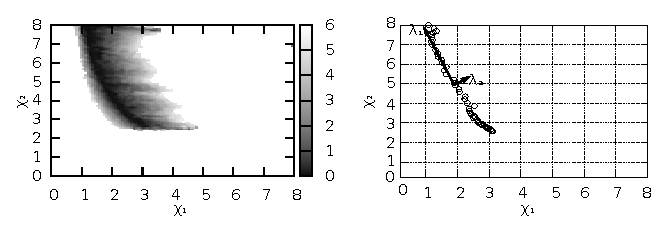
\includegraphics{DOFs.eps}}
\end{minipage}
\begin{minipage}[b]{0.5\linewidth}
 \centering
 \resizebox*{7.5cm}{!}{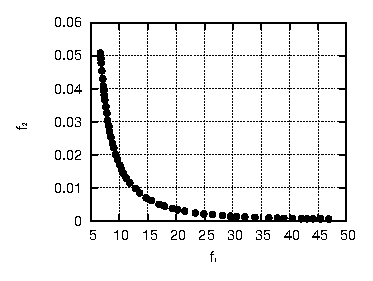
\includegraphics{Pareto.eps}}
\end{minipage}
\caption{Members of the Pareto front plotted on the design space (left) and objective space (right). For the pareto members the correlation described above is obvious.  Pareto members lay on a small band with respect to the above observations.}
\label{pareto_DOFs}
\end{figure}

EAs exploit the relationships between decision variables via rotating their design space in order to align it to the relations directions and by that influence the offspring probability distribution on the design space in order to maximise the probability of an individual to appear on the Pareto front. Regarding Crossover, since it takes place for each variable separately the probability distribution is bounded by a dof-dimentional hyber-cube (box for two objectives) aligned with the coordinate system it is applied on (fig \ref{xover}). To demonstrate how the probability distribution changes we use as an example 2 hypothetical parents plot the offspring probability distribution and based on that the probability of an individual to appear on the Pareto front(fig \ref{xover}). The probability of a individual to appear on the Pareto front is proportional to the length of the Pareto front interception line (fig \ref{xover}). For mutation, if the mutation probability is $p_m$ it is more probable to have a mutations happen on one of the axises of the coordinate system ($p_m$) and less probable as the number ($s$) of axises that have to simultaneously suffer mutation increases ($p_m^s$) (fig. \ref{mut}).      



\begin{figure}[h!]
\begin{minipage}[b]{0.5\linewidth}
 \centering
 \resizebox*{7.0cm}{!}{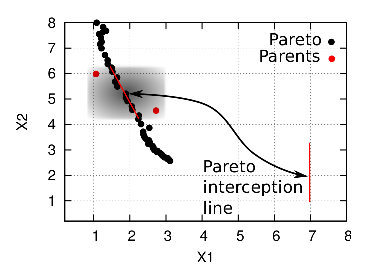
\includegraphics{DOFs_Xover2.eps}}
\end{minipage}
\begin{minipage}[b]{0.5\linewidth}
 \centering
 \resizebox*{7.0cm}{!}{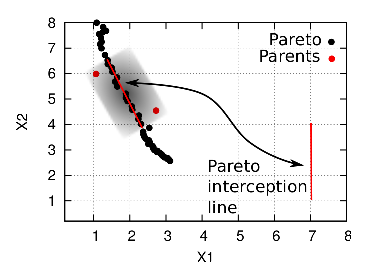
\includegraphics{DOFs_Xover.eps}}
\end{minipage}
\caption{Crossover offspring probability distribution bounding boxes as applied for original design plane (left) and the variable-relations-based rotated one (right). Pareto front interception line is significantly larger when crossover is applied on the rotated. "Extrapolation" magnitude and propability distribution in the bounding box depends on the crossover operator in use.}
\label{xover}
\end{figure}

The directions that describe the relations between design variables can be estimated at each generation via a statistical tool (principal component analysis -PCA) on current elite set and updated continuously as the elite set tents to approximate the actual pareto front. 

\begin{figure}[h!]
\begin{minipage}[b]{0.5\linewidth}
 \centering
 \resizebox*{7.0cm}{!}{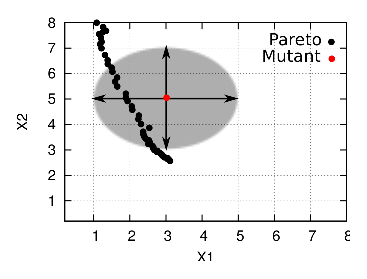
\includegraphics{DOFs_mut.eps}}
\end{minipage}
\begin{minipage}[b]{0.5\linewidth}
 \centering
 \resizebox*{7.0cm}{!}{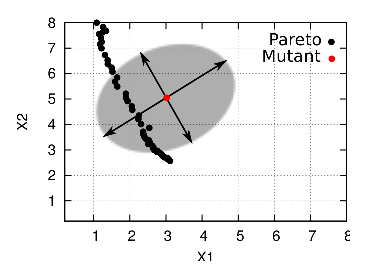
\includegraphics{DOFs_mut2.eps}}
\end{minipage}
\caption{Mutation offspring probability distribution as applied for original design variables (left) and the correlation based directions (right). Mutation in direction one is essential for improving the pareto representation quality and mutation on direction two to advance the current elite front towards the real pareto front. Both of them are equally valuable for an optimization procedure and the probability of them to happen decreases exponentially with the number of the correlated design variables.}
\label{mut}
\end{figure}



% ---------------------------------------------------------------------------
% ----------------------- end of thesis sub-document ------------------------
% ---------------------------------------------------------------------------